\documentclass[12pt,a4paper,oneside]{report}

% Essential Packages
\usepackage[utf8]{inputenc}
\usepackage[margin=1in]{geometry}
\usepackage{amsmath,amssymb,amsfonts}
\usepackage{graphicx}
\usepackage{booktabs}
\usepackage{multirow}
\usepackage{hyperref}
\usepackage{cite}
\usepackage[linesnumbered,ruled,vlined]{algorithm2e}
\usepackage{setspace}
\usepackage{caption}
\usepackage{subcaption}
\usepackage{fancyhdr}

\hypersetup{
    colorlinks=true,
    linkcolor=blue,
    citecolor=blue,
    urlcolor=blue
}

\onehalfspacing

\begin{document}

% ---------------------------------------------------------
% TITLE PAGE
% ---------------------------------------------------------
\begin{titlepage}
\centering
\vspace*{1cm}

{\Huge \textbf{Adaptive and Resource-Efficient Network Intrusion Detection for Previously Unseen Attacks in IoT Networks}\par}
\vspace{1.5cm}

{\Large \textbf{A Thesis Submitted in Partial Fulfillment of the Requirements for the Degree of}\par}
\vspace{0.5cm}
{\Large \textbf{Master of Technology (M.Tech)}\par}
\vspace{0.3cm}
{\large in Computer Science and Engineering / Cyber Security\par}

\vspace{2cm}
{\large \textbf{Submitted By:}\par}
{\Large \textbf{Sai Bhuvan}\par}

\vfill
{\large Department of Computer Science and Engineering\par}
\vspace{0.3cm}
{\large 2026\par}
\end{titlepage}

% ---------------------------------------------------------
% ABSTRACT
% ---------------------------------------------------------
\newpage
\pagenumbering{roman}
\chapter*{Abstract}
\addcontentsline{toc}{chapter}{Abstract}

Machine learning based Network Intrusion Detection Systems (NIDS) for the Internet of Things (IoT) are trained on a fixed set of attack classes and cannot recognise attacks outside that set. Adding a new attack class forces a trade-off on resource-constrained edge devices: full retraining is expensive in memory and compute, while incremental updates cause catastrophic forgetting of previously learned attacks. This thesis proposes a resource-efficient, replay-based continual learning framework that lets an edge NIDS learn previously unseen attacks while retaining earlier knowledge. Under a leave-one-attack-out protocol on the TON\_IoT dataset (211{,}043 flows), a Random Forest baseline with 97.2\% overall accuracy scores an F1 of 0.000 on each held-out attack (MITM, ransomware, XSS and backdoor). An unsupervised Isolation Forest provides a partial novelty signal, detecting 18.9\% of unseen MITM flows, and this signal triggers supervised adaptation. For rare attacks, a class-balanced replay buffer of 100 exemplars per class raises MITM F1 from 0.648 (naïve full retraining) to 0.977, while storing 99.3\% fewer samples and updating 11$\times$ faster. Static buffers, however, suffer up to 0.397 maximum forgetting under high-volume attacks. We therefore introduce a volume-aware Dynamic Replay rule that scales the per-class replay quota with the incoming attack volume, within fixed lower and upper memory bounds. Across three volumetric attacks, it reduces maximum forgetting by 20--36\% and average forgetting by up to 40\%, keeps novel-attack F1 above 0.997, preserves 96.8--97.6\% memory savings, and completes updates in under 0.1~s. A sensitivity analysis shows that even 25 exemplars per class learn MITM with an F1 of 0.980. These results demonstrate that selective, volume-aware retention, rather than large-scale storage, enables practical continual intrusion detection on constrained IoT devices.

\vspace{1cm}
\noindent \textbf{Keywords:} IoT Security, Network Intrusion Detection, Continual Learning, Catastrophic Forgetting, Experience Replay, Unseen Attacks, Resource-Efficient Machine Learning.

% ---------------------------------------------------------
% TABLE OF CONTENTS & LISTS
% ---------------------------------------------------------
\newpage
\tableofcontents

\newpage
\listoffigures

\newpage
\listoftables

% ---------------------------------------------------------
% CHAPTERS
% ---------------------------------------------------------
\newpage
\pagenumbering{arabic}

\chapter{Introduction}
\label{chap:introduction}

\section{Background and Context}
The pervasive deployment of the Internet of Things (IoT) has fundamentally transformed modern industrial automation, healthcare delivery, critical public infrastructure, and consumer smart environments. Modern IoT ecosystems are characterized by vast networks of interconnected edge devices—ranging from low-power smart sensors and microcontroller units to smart gateways and edge routers—that continuously acquire, process, and transmit telemetry data. However, the ubiquitous expansion of IoT infrastructure has outpaced traditional cybersecurity paradigms, introducing unprecedented vulnerabilities. Edge devices operate under severe hardware constraints, characterized by restricted volatile memory (RAM), limited non-volatile storage, low computational throughput, and tight thermal and battery energy budgets. Consequently, these devices represent attractive targets for malicious actors seeking to launch distributed denial-of-service (DDoS) botnets, ransomware deployments, credential exfiltration, and unauthorized lateral network movements.

To safeguard distributed IoT infrastructure, Network Intrusion Detection Systems (NIDS) have emerged as the foundational layer of cyber defense. Traditional signature-based detection systems rely on static rule databases; while effective against previously analyzed exploits, they fail catastrophically when confronted with zero-day attacks, modified payloads, or obfuscated traffic patterns. In response, Machine Learning (ML) and Deep Learning (DL) methodologies have been widely integrated into NIDS architectures to automatically discover complex non-linear signatures from high-dimensional network flow data. When trained on benchmark datasets such as TON\_IoT, modern supervised algorithms (e.g., Random Forests, Gradient Boosted Trees, and Deep Neural Networks) achieve near-perfect classification accuracies exceeding 98\% across known attack categories.

\section{The Core Dilemma: Static Models in Dynamic Environments}
Despite their high empirical accuracy under controlled laboratory benchmarks, conventional supervised NIDS operate under a rigid, flawed assumption: the \textbf{Closed-World Assumption}. Closed-world learning presupposes that the probability distribution of network traffic during operational deployment is strictly identical to the historical distribution observed during offline training ($\mathcal{P}_{test}(\mathbf{x}, y) = \mathcal{P}_{train}(\mathbf{x}, y)$).

In practical network deployments, this assumption is invalid. Adversarial tactics evolve continuously: zero-day vulnerabilities are weaponized, malware variants dynamically alter their payload heuristics, and targeted exploits—such as Man-in-the-Middle (MITM) session hijacking or stealthy backdoor compromises—emerge without historical precedent. When a closed-world supervised model encounters an out-of-distribution (OOD) novel attack, its mathematical formulation forces it to assign the new vector to one of its predefined known classes. As our preliminary experiments demonstrate, a baseline Random Forest model achieves an exact \textbf{0.000 F1-score} when confronted with an unobserved MITM or zero-day attack, misclassifying malicious payloads as benign traffic or generic denial-of-service flows.

To address zero-day vulnerabilities, the cybersecurity literature has historically explored two divergent paradigms, both of which suffer from severe practical limitations in IoT edge environments:
\begin{enumerate}
    \item \textbf{Unsupervised Anomaly Detection:} Unsupervised models (such as Isolation Forests or Deep Autoencoders) model the boundary of normal operational behavior and flag statistically deviant flows as anomalies. However, as demonstrated in our findings, unsupervised anomaly detectors suffer from high false-positive rates and low detection recall on nuanced attacks (e.g., yielding only 18.8\% detection recall on MITM flows). Furthermore, anomaly detectors provide binary alerts without classification granularity and cannot autonomously update downstream classifiers.
    \item \textbf{Offline Full Joint Retraining:} When a novel attack vector is identified and labeled by network administrators, the standard operational remedy is to aggregate the new attack data with the historical training corpus and retrain the classification model from scratch. In real-world edge IoT networks, this brute-force retraining paradigm is mathematically and physically infeasible. Storing tens of gigabytes of historical packet traces requires storage capacity that edge nodes do not possess. Moreover, complete retraining is computationally expensive, induces significant latency, causes thermal throttling, and introduces extreme class imbalance where massive historical datasets overwhelm small zero-day attack signatures.
\end{enumerate}

\section{The Plasticity-Stability Dilemma in Continual Learning}
Continual Learning (also termed Lifelong Learning) seeks to enable machine learning models to assimilate new knowledge from non-stationary data streams sequentially without degrading performance on previously acquired knowledge. The fundamental challenge governing continual learning is the \textbf{Plasticity-Stability Dilemma}:
\begin{itemize}
    \item \textbf{Plasticity:} The capacity of a learning system to readily adapt its internal parameters to acquire new representations and patterns from novel data distributions.
    \item \textbf{Stability:} The capacity of the system to preserve its historical representations and retain high accuracy on legacy tasks over time.
\end{itemize}

When standard models are fine-tuned exclusively on newly emerging attack data, they prioritize plasticity at the total expense of stability, succumbing to \textbf{Catastrophic Forgetting}. The optimization trajectory aggressively alters model decision boundaries to minimize empirical risk on the new data, thereby obliterating the boundaries previously constructed for historical attacks. Consequently, while the updated model successfully learns the new attack, it completely loses its ability to recognize basic historical threats (e.g., DDoS or Password cracking).

While experience replay (replaying a subset of historical samples alongside new samples) has emerged as an effective countermeasure to catastrophic forgetting, existing replay literature assumes either infinite memory buffers or arbitrary static buffer sizes. As uncovered in this thesis, a fixed static replay buffer creates a volatile adaptation-retention trade-off: when a large volumetric attack (e.g., XSS or Backdoor with thousands of packets) hits the network, it severely outnumbers a static buffer, triggering a catastrophic forgetting spike where accuracy on historical classes degrades by nearly 40\%.

\section{Problem Statement}
This research addresses the following formal problem statement:
\begin{quote}
\textit{``How can we design, formulate, and validate an autonomous, resource-efficient Continual Learning framework for IoT Network Intrusion Detection that reliably identifies previously unobserved zero-day cyber threats, rapidly assimilates confirmed novel attack classes with high plasticity, and dynamically mitigates catastrophic forgetting across varying incoming attack volumes, all while adhering to the strict memory and computational constraints of edge IoT hardware?''}
\end{quote}

\section{Research Questions}
To resolve this problem, the thesis investigates five specific research questions:
\begin{itemize}
    \item \textbf{RQ1 (Supervised Failure Mode):} How severely do state-of-the-art closed-world supervised intrusion detection models fail when deployed against previously unobserved network attack classes?
    \item \textbf{RQ2 (Anomaly Detection Utility):} To what extent can unsupervised anomaly detection (specifically Isolation Forests) reliably isolate zero-day network traffic without producing prohibitive false alarm rates?
    \item \textbf{RQ3 (Replay Memory Sensitivity):} How does historical memory buffer capacity govern the empirical Pareto trade-off between legacy knowledge retention and resource consumption?
    \item \textbf{RQ4 (Volumetric Attack Dynamics):} Why do static-sized replay buffers fail during the assimilation of high-volume incoming attacks, and what are the mechanics of the resulting catastrophic forgetting spikes?
    \item \textbf{RQ5 (Dynamic Allocation Efficacy):} Can an autonomous, volume-aware dynamic replay allocation strategy mathematically stabilize knowledge retention and eliminate forgetting spikes while maintaining extreme ($>96\%$) memory savings?
\end{itemize}

\section{Research Hypotheses}
The investigations in this thesis are guided by the following formal hypotheses:
\begin{itemize}
    \item \textbf{H1:} Closed-world supervised tree ensembles yield exactly zero recall ($F1 = 0.00$) for unobserved attack vectors, validating the theoretical detection deficit.
    \item \textbf{H2:} Unsupervised anomaly detection provides an effective preliminary filter for out-of-distribution traffic but cannot serve as a standalone replacement for supervised multi-class classification.
    \item \textbf{H3:} Memory storage overhead can be compressed by over 95\% relative to full joint retraining without causing legacy catastrophic forgetting, provided a minimum representative exemplar floor is maintained.
    \item \textbf{H4:} A dynamic replay allocation rule that scales historical exemplar sampling proportionally to incoming novel attack volume will structurally suppress maximum catastrophic forgetting spikes relative to rigid static buffers.
\end{itemize}

\section{Key Contributions of the Thesis}
The primary contributions of this thesis are as follows:
\begin{enumerate}
    \item \textbf{Comprehensive Empirical Mapping of the Zero-Day Failure Mode:} We establish a rigorous empirical baseline on the TON\_IoT dataset, isolating four distinct attack vectors (MITM, Ransomware, XSS, Backdoor) and quantifying the exact catastrophic forgetting dynamics across baseline, unsupervised, and continual learning models.
    \item \textbf{Discovery of the Full Retraining Class Imbalance Trap:} We empirically prove that full joint retraining—the assumed industry gold standard—actually harms novel attack acquisition on compact zero-day exploits (achieving only 0.648 F1 on MITM), whereas our balanced replay framework achieves 0.977 F1 (+32.9\% improvement).
    \item \textbf{Formulation of a Novel Dynamic Volume-Aware Replay Framework:} We design and implement an explainable, deterministic dynamic allocation algorithm:
    \begin{equation*}
    k_{dynamic} = \max\left( k_{min}, \min\left( k_{max}, \left\lfloor \frac{M \cdot \alpha}{K} \right\rfloor \right) \right)
    \end{equation*}
    which adaptively balances the plasticity-stability equilibrium based on the incoming novelty volume.
    \item \textbf{Empirical Mitigation of Maximum Catastrophic Forgetting Spikes:} Across four distinct attack classes with varying volumes, our dynamic framework slashes maximum catastrophic forgetting on hardest legacy classes by 35.8\% (capping drops below 0.25 compared to 0.397 in static buffers).
    \item \textbf{Ultra-Low Resource Footprint for Edge IoT Nodes:} The framework maintains extreme memory reduction ($96.8\%$ to $99.3\%$ reduction in historical sample storage) and achieves sub-0.085 second adaptation latency, enabling genuine real-time, on-device execution on edge gateways.
    \item \textbf{Formal Sustainability and UN SDG Alignment:} We contextualize the computational efficiencies of the framework within the United Nations Sustainable Development Goals (SDG 9, SDG 11, and SDG 12), quantifying energy and carbon reductions compared to brute-force retraining.
\end{enumerate}

\section{Thesis Organization}
The remainder of this thesis is structured as follows:
\begin{itemize}
    \item \textbf{Chapter~\ref{chap:literature_review}} provides a comprehensive review of related literature in machine learning for NIDS, zero-day anomaly discovery, continual learning paradigms, and experience replay limitations.
    \item \textbf{Chapter~\ref{chap:system_model}} details the system architecture, mathematical threat model, edge hardware constraints, and the formal formulation of the plasticity-stability trade-off.
    \item \textbf{Chapter~\ref{chap:proposed_framework}} presents the mathematical derivation, buffer management mechanics, and algorithmic implementation of the proposed Dynamic Continual Learning framework.
    \item \textbf{Chapter~\ref{chap:experimental_setup}} outlines the experimental methodology, TON\_IoT dataset characteristics, feature preprocessing, zero-day simulation protocol, and formal continual learning evaluation metrics.
    \item \textbf{Chapter~\ref{chap:results_and_discussion}} presents the exhaustive empirical findings, multi-attack comparison tables, publication-quality visualizations, and in-depth discussions.
    \item \textbf{Chapter~\ref{chap:conclusion}} concludes the thesis, summarizing key theoretical and empirical contributions, acknowledging limitations, and outlining future research directions.
\end{itemize}

\chapter{Literature Review and Related Work}
\label{chap:literature_review}

\section{Machine Learning in Network Intrusion Detection}
Network Intrusion Detection Systems (NIDS) constitute an indispensable component of defensive cyber operations. Over the past decade, the rapid proliferation of high-throughput network architectures and the sophistication of encrypted adversarial tactics have rendered conventional signature-matching systems (e.g., Snort, Suricata) insufficient against polymorphous exploits. Consequently, extensive research has focused on applying Machine Learning (ML) and Deep Learning (DL) to statistical packet flow analytics.

Traditional supervised algorithms—including Support Vector Machines (SVM), k-Nearest Neighbors (k-NN), Decision Trees, and Naive Bayes—were initially leveraged on historical intrusion datasets such as KDD-CUP99 and NSL-KDD. However, these classical datasets have been widely criticized in literature for unrealistic traffic distributions, outdated attack primitives, and severe artificial class redundancies. 

With the emergence of contemporary benchmarks such as UNSW-NB15, CIC-IDS2017, and particularly the **TON\_IoT** dataset, researchers transitioned toward advanced tree-ensemble methodologies, notably Random Forests (RF), XGBoost, and LightGBM. Ensemble tree methods consistently exhibit state-of-the-art performance on tabular network metadata (e.g., packet header statistics, inter-arrival times, byte rates, and TCP flag counts). Their superior performance is driven by their capacity to capture non-linear feature interactions, natural resistance to numerical feature scaling disparities, and resilience against multi-collinearity. In static benchmarks, Random Forest architectures routinely attain over 97\% classification accuracy with low false-alarm ratios.

Despite these achievements, a critical deficiency persists across the vast majority of supervised NIDS literature: models are evaluated strictly under static, stationary test splits. In real-world deployment environments, network distributions are non-stationary, and supervised classifiers operate under a closed-world assumption that blinds them to out-of-distribution attacks.

\section{Zero-Day Threat Discovery and Anomaly Detection}
To overcome the closed-world limitation of supervised learning, researchers have extensively explored unsupervised and semi-supervised anomaly detection. These frameworks train exclusively on benign baseline traffic, aiming to model the normal operational manifold of the network:
\begin{enumerate}
    \item \textbf{Statistical and Distance-Based Detectors:} Methods such as One-Class Support Vector Machines (OC-SVM) and Local Outlier Factor (LOF) delineate high-density regions of benign behavior. While mathematically rigorous, their computational complexity scales quadratically with dataset volume ($\mathcal{O}(N^2)$), rendering them impractical for high-speed IoT gateway monitoring.
    \item \textbf{Tree-Based Ensembles (Isolation Forests):} Proposed by Liu et al., Isolation Forests isolate anomalies by recursively partitioning feature space using random orthogonal hyperplanes. Since anomalies are mathematically few and qualitatively divergent, they exhibit significantly shorter average path lengths in binary isolation trees. Isolation Forests achieve linear computational complexity ($\mathcal{O}(N \log N)$) and low memory consumption, making them the leading candidate for resource-constrained edge computing.
    \item \textbf{Deep Autoencoders and Variational Autoencoders (VAEs):} Deep neural autoencoders reconstruct benign network features through an informational bottleneck. Flows yielding high reconstruction errors are flagged as anomalies. While capable of learning rich latent representations, deep autoencoders require extensive graphics processing unit (GPU) acceleration and hyperparameter tuning, which exceeds the thermal and architectural capabilities of edge microcontrollers.
\end{enumerate}

Despite their theoretical appeal for zero-day threat discovery, unsupervised anomaly detectors exhibit severe practical drawbacks in operational settings. First, normal IoT traffic is frequently noisy and bursting (e.g., periodic sensor updates, network reconnections), leading to unacceptable false-positive rates that trigger alert fatigue for security operations teams. Second, anomaly detectors only generate binary alarm signals; they lack multi-class discriminatory granularity, cannot distinguish between attack types (e.g., differentiating benign misconfigurations from active MITM exploits), and possess no native mechanism to update downstream classification engines.

\section{Continual Learning Paradigms}
Continual Learning (also known as Lifelong Learning or Incremental Learning) provides the foundational mathematical framework to overcome static model obsolescence. Continual learning algorithms are categorized into three primary structural paradigms:

\subsection{Regularization-Based Approaches}
Regularization methods prevent catastrophic forgetting by penalizing modifications to model parameters that were critical for historical tasks. 
\begin{itemize}
    \item \textbf{Elastic Weight Consolidation (EWC):} Proposed by Kirkpatrick et al., EWC calculates the diagonal elements of the Fisher Information Matrix to identify parameter sensitivity. When updating the model on task $T_2$, quadratic penalties are applied to parameter shifts along high-curvature dimensions corresponding to task $T_1$.
    \item \textbf{Synaptic Intelligence (SI):} Zenke et al. introduced path-integral metrics to measure parameter importance online during gradient descent trajectories.
\end{itemize}
While computationally elegant and requiring zero historical sample storage, regularization techniques suffer from two fatal weaknesses in cybersecurity applications: they struggle under long task sequences (as parameter capacity quickly saturates) and are fundamentally restricted to differentiable neural networks, precluding their use with high-performing, resource-efficient tree ensemble models.

\subsection{Parameter Isolation and Architecture-Expanding Approaches}
Parameter isolation methods allocate dedicated sub-networks or dynamically expand model architecture when encountering new tasks (e.g., Progressive Neural Networks, PackNet). While completely eliminating catastrophic forgetting, the architectural complexity and memory footprint scale linearly with the number of encountered tasks ($\mathcal{O}(T)$), violating the rigid hardware constraints of IoT devices.

\subsection{Replay-Based Approaches (Experience Replay)}
Replay methods mitigate catastrophic forgetting by retaining or generating representative historical exemplars and re-exposing them to the learning algorithm during new task optimization. Experience replay remains the most empirically robust continual learning strategy in non-stationary environments.
\begin{itemize}
    \item \textbf{Generative Replay:} Generative Adversarial Networks (GANs) or diffusion models synthesize pseudo-historical samples. However, training generative networks on edge IoT hardware is computationally prohibitive and prone to mode collapse.
    \item \textbf{Exemplar Replay:} Historical training samples are preserved in an episodic replay buffer. During novel task learning, exemplars are combined with new task data. Replay buffers are natively compatible with both neural architectures and ensemble decision trees.
\end{itemize}

\section{Replay in Cybersecurity and the Memory Bottleneck}
Recent pioneering work by researchers has begun evaluating continual learning within the cybersecurity domain. Notably, the landmark study \textit{``Replay or Regret: Evaluating Continual Learning Methods for Robust Intrusion Detection''} systematically benchmarked regularization and replay methods across multi-class network traffic streams. The authors unequivocally demonstrated that rehearsal-based replay methods consistently outperform parameter regularization across network intrusion benchmarks.

However, existing literature universally relies on one of two flawed memory assumptions:
\begin{enumerate}
    \item \textbf{The Infinite Buffer / Full Retraining Assumption:} Models assume access to an unconstrained centralized repository where all historical training data is permanently retained. Full joint retraining is triggered whenever new attacks are identified. As previously emphasized, this brute-force approach requires storing hundreds of thousands of high-dimensional flow records, which is impossible on edge IoT devices with constrained flash storage.
    \item \textbf{The Arbitrary Static Buffer Assumption:} When memory limits are imposed, researchers uniformly assign an arbitrary, fixed static buffer size (e.g., $k = 50$ or $k = 100$ samples per class).
\end{enumerate}

\section{Critical Research Gaps in Contemporary Literature}
A rigorous synthesis of the related literature reveals three critical research gaps:
\begin{itemize}
    \item \textbf{Research Gap 1: Disconnected Zero-Day Detection and Model Adaptation:} Existing systems either focus on detecting anomalies or on incremental training, but fail to integrate both into an autonomous, closed-loop pipeline where isolated zero-day anomalies seamlessly trigger on-device adaptation.
    \item \textbf{Research Gap 2: The Full Retraining Imbalance Vulnerability:} Prior literature assumes full retraining is the optimal performance ceiling. However, the severe class imbalance induced when small zero-day attack batches are submerged within massive historical datasets has been largely overlooked.
    \item \textbf{Research Gap 3: Volumetric Vulnerability of Static Buffers:} Contemporary continual NIDS literature assumes static memory buffers. The vulnerability of fixed buffers when confronted with varying incoming attack volumes—where massive attacks overwhelm the buffer and trigger severe catastrophic forgetting spikes—remains unaddressed.
\end{itemize}

This thesis directly bridges these critical gaps by architecting an integrated, volume-aware Dynamic Continual Learning framework tailored specifically for resource-constrained IoT edge environments.

\chapter{System Model and Problem Formulation}
\label{chap:system_model}

\section{Edge IoT Network Architecture and Threat Model}
\subsection{Deployment Topology}
The target deployment environment considered in this thesis corresponds to a distributed Edge IoT architecture, commonly encountered in smart manufacturing, healthcare monitoring, and intelligent municipal infrastructure. The network architecture consists of three hierarchical layers:
\begin{enumerate}
    \item \textbf{Perception and Sensor Layer:} Microcontroller-driven smart endpoints (e.g., environmental monitors, medical telemetry sensors, industrial PLCs) that continuously capture physical observations and transmit digitized telemetry using lightweight application protocols (e.g., MQTT, CoAP, Modbus).
    \item \textbf{Edge Computing Layer:} Intermediate network aggregation hardware, such as edge gateways, industrial access routers, and smart border hubs. These devices aggregate heterogeneous sensor streams, perform preliminary data filtering, and host the real-time Network Intrusion Detection System (NIDS).
    \item \textbf{Centralized Management / Cloud Layer:} Upstream enterprise security operations centers (SOC) that manage long-term threat intelligence, security policy updates, and human-in-the-loop incident auditing.
\end{enumerate}

\subsection{Threat Model and Adversarial Capabilities}
Adversaries targeting edge IoT networks exhibit diverse technical objectives and traffic generation profiles:
\begin{itemize}
    \item \textbf{Stealthy / Low-Volume Adversaries (e.g., MITM):} Malicious actors that deploy ARP spoofing or DNS poisoning to silently intercept, inspect, or tamper with sensory payloads without disrupting network connectivity. These attacks generate minimal anomalous traffic volume ($\sim$100--200 packets), deliberately evading rate-limiting volumetric defenses.
    \item \textbf{Exploitative / Persistent Adversaries (e.g., Ransomware, Password Brute-Force):} Adversaries seeking to compromise edge device credentials or encrypt local filesystems, generating sustained bursts of credential-guessing or SMB/RPC packet flows ($\sim$1,000--3,000 packets).
    \item \textbf{Volumetric / Aggressive Adversaries (e.g., XSS, Backdoor, DDoS):} High-volume compromise campaigns involving automated vulnerability scanning, injection attacks, and reverse shell beacons. These attacks generate thousands of network flows ($\sim$3,000--4,000 packets), presenting sudden bursts of novel traffic.
\end{itemize}

\section{Mathematical Formulation of the NIDS Problem}
Let raw network traffic be represented as a continuous, time-ordered sequence of packet flows $\mathcal{S} = \{\mathbf{f}_1, \mathbf{f}_2, \dots, \mathbf{f}_t, \dots\}$. Each flow $\mathbf{f}_t$ is summarized by a feature extraction preprocessor into a real-valued feature vector $\mathbf{x}_t \in \mathcal{X} \subset \mathbb{R}^d$, where $d$ denotes the feature dimensionality (including statistical flow metrics such as duration, packet counts, inter-arrival times, TCP flags, and protocol indicators).

\subsection{Closed-World Supervised Formulation}
Under the standard closed-world formulation, the intrusion detection model is trained offline on a static historical dataset:
\begin{equation}
\mathcal{D}_{train} = \{(\mathbf{x}_i, y_i)\}_{i=1}^{N}, \quad \mathbf{x}_i \in \mathcal{X}, \quad y_i \in \mathcal{C}_{known}
\end{equation}
where $\mathcal{C}_{known} = \{1, 2, \dots, K\}$ denotes the set of $K$ known attack classes (e.g., Benign, DDoS, Scanning, Password, etc.). 

A supervised multi-class classifier $f_{\theta}: \mathcal{X} \rightarrow \mathcal{C}_{known}$ is trained by minimizing the empirical risk over $\mathcal{D}_{train}$:
\begin{equation}
\theta^* = \arg\min_{\theta} \frac{1}{N} \sum_{i=1}^{N} \mathcal{L}(f_{\theta}(\mathbf{x}_i), y_i)
\end{equation}
where $\mathcal{L}$ denotes the multi-class loss function (such as Gini impurity minimization in Random Forests or cross-entropy loss).

\subsection{Open-World Zero-Day Vulnerability}
In an operational deployment, network flows are drawn from an open-world distribution:
\begin{equation}
\mathcal{P}_{open}(\mathbf{x}, y) = (1 - \pi) \mathcal{P}_{known}(\mathbf{x}, y) + \pi \mathcal{P}_{novel}(\mathbf{x}, y)
\end{equation}
where $\pi \in [0, 1]$ represents the probability of encountering a novel, unobserved zero-day attack class $y^* \notin \mathcal{C}_{known}$.

Because the decision space of the closed-world classifier $f_{\theta}$ is strictly bounded by $\mathcal{C}_{known}$, the probability simplex satisfies:
\begin{equation}
\sum_{k \in \mathcal{C}_{known}} P(y = k \mid \mathbf{x}) = 1.0, \quad \forall \mathbf{x} \in \mathcal{X}
\end{equation}
Consequently, when a novel packet $\mathbf{x}_{novel} \sim \mathcal{P}_{novel}$ enters the system:
\begin{equation}
f_{\theta}(\mathbf{x}_{novel}) \in \mathcal{C}_{known} \implies \text{Error Guaranteed}
\end{equation}
The closed-world classifier is mathematically incapable of identifying the attack as novel, forcing an immediate false-negative or misclassification error.

\section{The Mechanics of Catastrophic Forgetting in Decision Tree Ensembles}
While catastrophic forgetting is typically analyzed within gradient-based neural networks (where weight updates overwrite historical orthogonal features), it is equally devastating in non-parametric tree ensembles such as Random Forests. 

A Random Forest comprises an ensemble of $B$ independent decision trees $\{T_b\}_{b=1}^{B}$. For each tree, recursive binary splitting selects the feature $j$ and threshold $\tau$ that maximize the impurity reduction $\Delta I$:
\begin{equation}
\Delta I(s, j, \tau) = I(s) - \frac{|s_L|}{|s|} I(s_L) - \frac{|s_R|}{|s|} I(s_R)
\end{equation}
where $I(s)$ represents the Gini impurity of node $s$:
\begin{equation}
I(s) = 1 - \sum_{k=1}^{K} p_k^2
\end{equation}
and $p_k$ is the empirical fraction of class $k$ samples present at node $s$.

\subsection{Why Fine-Tuning Only on New Attacks Destroys Legacy Boundaries}
When an updated batch containing solely novel attack samples $\mathcal{D}_{novel}$ is presented to the model without historical context:
\begin{equation}
p_{novel} \rightarrow 1.0, \quad p_k \rightarrow 0 \quad (\forall k \in \mathcal{C}_{known})
\end{equation}
The tree construction algorithm optimizes feature splits solely to isolate the novel class from residual noise. All existing internal split nodes that previously partitioned historical classes (e.g., distinguishing DDoS from Benign traffic) are eradicated because historical classes have zero empirical presence in the optimization batch. Consequently, legacy accuracy drops catastrophically to zero.

\subsection{The Imbalance Vulnerability of Static Buffers}
When a fixed static buffer $\mathcal{B}_{static}$ is utilized with a quota of $k_{static}$ samples per class, the total historical memory size is $|\mathcal{B}_{static}| = K \cdot k_{static}$. 

If a novel volumetric attack arrives with $M = |\mathcal{D}_{novel}|$ samples:
\begin{equation}
\text{Imbalance Ratio } \rho = \frac{M}{K \cdot k_{static}}
\end{equation}
\begin{itemize}
    \item When $\rho \ll 1$ (e.g., MITM attack, $M \approx 180$, $K \cdot k_{static} = 900$, $\rho = 0.20$): The historical classes maintain dominant representation. The tree splits preserve historical boundaries, and forgetting remains negligible ($\mathcal{F}_{max} \approx 0.06$).
    \item When $\rho \gg 1$ (e.g., XSS or Backdoor, $M \approx 3,500$, $K \cdot k_{static} = 900$, $\rho = 3.88$): The novel attack dominates the training set by nearly 4:1. During tree construction, the greedy split algorithm heavily favors splitting features that pure-classify the massive novel class, sacrificing historical boundary purity and causing severe catastrophic forgetting spikes ($\mathcal{F}_{max} \approx 0.40$).
\end{itemize}

This mathematical reality proves that fixed static buffers are fundamentally flawed for intrusion detection: the buffer must dynamically scale to neutralize the imbalance ratio $\rho \approx 1.0$.

\chapter{Proposed Methodology: Dynamic Continual Learning Framework}
\label{chap:proposed_framework}

\section{Architecture Overview}
The proposed architecture addresses the fundamental vulnerability of static Machine Learning-based Network Intrusion Detection Systems (NIDS) deployed in resource-constrained IoT environments: their complete blindness to novel zero-day attack vectors and the prohibitive cost of full offline retraining. 

As illustrated in Figure~\ref{fig:framework_architecture}, the framework operates via a dual-stage closed-loop pipeline comprising:
\begin{enumerate}
    \item \textbf{Anomalous Vector Isolation (Stage 1):} High-entropy, out-of-distribution network packets are flagged without supervision using an Isolation Forest anomaly filter.
    \item \textbf{Dynamic Continual Adaptation Engine (Stage 2):} Once confirmed and labeled by network telemetry, novel attack traffic is incrementally absorbed into the active classifier using our resource-efficient \textbf{Dynamic Replay Buffer}.
\end{enumerate}

\begin{figure}[htbp]
\centering
\fbox{
\begin{minipage}{0.9\textwidth}
\centering
\vspace{0.3cm}
\textbf{\large Closed-Loop Dynamic Continual Learning Architecture}\\[0.3cm]
$\mathbf{x}_t \longrightarrow$ \framebox{Stage 1: Isolation Forest Anomaly Screener} $\longrightarrow$ [Anomaly Flagged / Out-of-Distribution]\\
$\downarrow$\\
\framebox{Dynamic Quota Allocator: $k = \max(k_{min}, \lfloor M / K \rfloor)$} $\longleftarrow$ [Incoming Novel Batch $\mathcal{D}_{novel}$]\\
$\downarrow$\\
\framebox{Historical Exemplar Replay Buffer $\mathcal{B}_{dynamic}$} $\oplus$ \framebox{Novel Threat Batch $\mathcal{D}_{novel}$}\\
$\downarrow$\\
\framebox{Continual Retraining Engine: $\mathcal{D}_{adapt}$} $\longrightarrow$ \textbf{Updated Resilient Model $f_{\theta'}$}\\[0.3cm]
\end{minipage}
}
\caption{Architectural block diagram of the proposed dual-stage adaptive intrusion detection framework, showcasing autonomous anomaly screening and volume-aware dynamic replay synthesis.}
\label{fig:framework_architecture}
\end{figure}

\section{Stage 1: Unsupervised Zero-Day Anomaly Screening}
The first stage of the defensive pipeline operates as an online anomaly filter directly on the ingress telemetry stream.

\subsection{Isolation Forest Formulation}
Let benign network traffic baseline samples be denoted as $\mathcal{X}_{benign} \subset \mathbb{R}^d$. An Isolation Forest comprising an ensemble of $T$ binary isolation trees $\{h_t\}_{t=1}^{T}$ is constructed. Each tree recursively splits the feature space by randomly selecting a feature dimension $j \in \{1, \dots, d\}$ and choosing a split value uniformly within the feature range $[x_{j}^{min}, x_{j}^{max}]$.

The isolation anomaly score $s(\mathbf{x}, n)$ for an incoming flow $\mathbf{x}$ evaluated over a dataset of size $n$ is defined as:
\begin{equation}
s(\mathbf{x}, n) = 2^{-\frac{\mathbb{E}(h(\mathbf{x}))}{c(n)}}
\end{equation}
where $\mathbb{E}(h(\mathbf{x}))$ denotes the average path length across the $T$ isolation trees, and $c(n)$ is the average path length of unsuccessful searches in a Binary Search Tree (BST):
\begin{equation}
c(n) = 2 \ln(n - 1) + 0.5772156649 \text{ (Euler's constant)} - \frac{2(n - 1)}{n}
\end{equation}

When $s(\mathbf{x}, n) \rightarrow 1.0$, the sample is isolated near the root with short path lengths, indicating that the network packet exhibits abnormal statistical characteristics. Flows exceeding an empirical threshold $\tau_{anomaly}$ are isolated and routed to the quarantine adaptation queue.

\section{Stage 2: Mathematical Formulation of Dynamic Replay}
Let $\mathcal{D}_{train} = \{(\mathbf{x}_i, y_i)\}_{i=1}^{N}$ denote the historical baseline network dataset containing known traffic classes $\mathcal{C}_{known} = \{1, 2, \dots, K\}$. A base supervised classifier $f_{\theta}: \mathcal{X} \rightarrow \mathcal{C}_{known}$ is initially optimized on $\mathcal{D}_{train}$.

When a novel attack vector $\mathcal{C}_{novel} = \{K+1\}$ appears in the IoT network, let $\mathcal{D}_{novel} = \{(\mathbf{x}_j, y_j)\}_{j=1}^{M}$ represent the incoming batch of novel attack signatures, where $M = |\mathcal{D}_{novel}|$.

\subsection{The Memory Footprint Challenge in IoT Edge Nodes}
Traditional continual learning either attempts full historical joint retraining on $\mathcal{D}_{train} \cup \mathcal{D}_{novel}$ (which requires maintaining $N \gg 10^5$ samples on local non-volatile storage) or relies on a small static buffer $\mathcal{B}_{static}$ containing a fixed quota $k_{static}$ samples per class ($|\mathcal{B}_{static}| = K \cdot k_{static}$). 

As demonstrated by our empirical findings, when the incoming attack volume $M$ significantly exceeds the fixed buffer capacity ($M \gg K \cdot k_{static}$), the decision boundaries of the tree ensemble are overwhelmed by the new majority class, resulting in severe \textit{maximum catastrophic forgetting} on historical classes.

\subsection{Dynamic Volume-Aware Replay Allocation Rule}
To mathematically prevent class imbalance during incremental tree construction while strictly bounding memory consumption, we introduce the volume-aware Dynamic Replay Allocation function $\Phi(M, K)$:

\begin{equation}
k_{dynamic} = \max\left( k_{min}, \min\left( k_{max}, \left\lfloor \frac{M \cdot \alpha}{K} \right\rfloor \right) \right)
\label{eq:dynamic_rule}
\end{equation}

Where:
\begin{itemize}
    \item $k_{min}$ is the guaranteed retention floor ($k_{min} = 100$ samples per known class), preventing catastrophic forgetting on low-volume attacks.
    \item $k_{max}$ is the physical hardware memory ceiling imposed by the IoT device's RAM/flash budget.
    \item $K = |\mathcal{C}_{known}|$ is the total number of known classes currently managed by the model.
    \item $\alpha \in [1.0, 1.2]$ is the class balance scaling multiplier, ensuring the historical buffer matches or slightly exceeds the incoming novelty volume in aggregate.
\end{itemize}

The dynamic historical replay buffer $\mathcal{B}_{dynamic}$ is then populated via stratified representative sampling:
\begin{equation}
\mathcal{B}_{dynamic} = \bigcup_{c \in \mathcal{C}_{known}} \mathcal{S}_{c}\left(\mathcal{D}_{train}^{(c)}, k_{dynamic}\right)
\end{equation}
where $\mathcal{S}_{c}(\cdot, k)$ extracts $k$ representative exemplars from historical class $c$.

The updated model $f_{\theta'}$ is subsequently trained on the balanced adaptation set:
\begin{equation}
\mathcal{D}_{adapt} = \mathcal{B}_{dynamic} \cup \mathcal{D}_{novel}
\end{equation}

\section{Algorithmic Workflow}

Algorithm~\ref{alg:dynamic_replay} details the exact operational execution flow executed on the edge gateway when novel threat signatures are assimilated.

\begin{algorithm}[H]
\caption{Dynamic Continual Learning Adaptation for IoT NIDS}
\label{alg:dynamic_replay}
\KwIn{Incoming novelty batch $\mathcal{D}_{novel}$, Historical repository $\mathcal{D}_{train}$, Known classes $\mathcal{C}_{known}$, Min buffer $k_{min}$, Max cap $k_{max}$}
\KwOut{Adapted Multi-Class Model $f_{\theta'}$, Adaptation Metadata $\mathcal{M}$}

$M \leftarrow |\mathcal{D}_{novel}|$\;
$K \leftarrow |\mathcal{C}_{known}|$\;

\tcp{Step 1: Compute Dynamic Allocation Quota}
$k_{dynamic} \leftarrow \max\left( k_{min}, \min\left( k_{max}, \lfloor M / K \rfloor \right) \right)$\;

\tcp{Step 2: Assemble Dynamic Replay Buffer}
$\mathcal{B} \leftarrow \emptyset$\;
\ForEach{$c \in \mathcal{C}_{known}$}{
    $\mathcal{D}_c \leftarrow \{(\mathbf{x}, y) \in \mathcal{D}_{train} \mid y = c\}$\;
    $\mathcal{B}_c \leftarrow \text{Sample}(\mathcal{D}_c, \min(k_{dynamic}, |\mathcal{D}_c|))$\;
    $\mathcal{B} \leftarrow \mathcal{B} \cup \mathcal{B}_c$\;
}

\tcp{Step 3: Synthesize Balanced Adaptation Corpus}
$\mathcal{D}_{adapt} \leftarrow \mathcal{B} \cup \mathcal{D}_{novel}$\;

\tcp{Step 4: Execute Fast On-Device Retraining}
$start\_time \leftarrow \text{GetCurrentTime}()$\;
$f_{\theta'} \leftarrow \text{TrainEnsemble}(\mathcal{D}_{adapt})$\;
$elapsed \leftarrow \text{GetCurrentTime}() - start\_time$\;

\tcp{Step 5: Record Adaptation Metadata}
$\mathcal{M} \leftarrow \{|\mathcal{B}|, \text{MemoryReduction}, elapsed\}$\;
\Return{$f_{\theta'}, \mathcal{M}$}
\end{algorithm}

\section{Computational Complexity and Resource Efficiency for Edge Nodes}
The computational complexity of standard Random Forest training on $N$ samples with $d$ features and $B$ trees is:
\begin{equation}
\mathcal{O}_{\text{full}} = B \cdot d \cdot N \log N
\end{equation}
Under our Dynamic Replay framework, the effective sample volume during adaptation is reduced from $N \approx 1.28 \times 10^5$ to $N_{adapt} = |\mathcal{B}_{dynamic}| + M \approx 1.8 \times 10^3 \text{ to } 7.5 \times 10^3$.

The computational complexity under adaptation reduces to:
\begin{equation}
\mathcal{O}_{\text{dynamic}} = B \cdot d \cdot N_{adapt} \log N_{adapt}
\end{equation}
Because $N_{adapt} \ll N$, this represents a theoretical speedup exceeding an order of magnitude:
\begin{equation}
\text{Speedup} \approx \frac{N \log N}{N_{adapt} \log N_{adapt}} \approx 10\times \text{ to } 25\times
\end{equation}
This theoretical reduction directly manifests in our empirical runtimes, where model adaptation completes in under $0.085$ seconds on edge CPU hardware.

\chapter{Empirical Evaluation and In-Depth Discussion}
\label{chap:results_and_discussion}

\section{Experimental Methodology and Setup}
All experimental benchmarks were conducted on the benchmark \textbf{TON\_IoT} network intrusion dataset, extracted from an active edge IoT testbed containing heterogeneous cyber threats and benign sensory network flows. To simulate zero-day deployment conditions, four distinct attack vectors representing varying volumetric characteristics were systematically quarantined during baseline training:
\begin{enumerate}
    \item \textbf{Man-in-the-Middle (MITM):} Low-volume, targeted exploit ($\sim$180 adaptation packets).
    \item \textbf{Ransomware:} Medium-volume, persistent protocol exploitation ($\sim$2,850 adaptation packets).
    \item \textbf{Cross-Site Scripting (XSS):} High-volume web application vector ($\sim$2,900 adaptation packets).
    \item \textbf{Backdoor:} High-volume administrative compromise vector ($\sim$3,730 adaptation packets).
\end{enumerate}

To strictly guarantee the absence of data snooping or optimistic leakage, an untouched 80\% holdout evaluation partition was quarantined for each quarantined novel attack class, while historical retention was continuously measured against the untouched test set of known legacy classes.

\section{Evaluation Metrics}
To rigorously quantify the trade-off between knowledge acquisition, memory conservation, and catastrophic forgetting, we evaluate models along six standardized axes:
\begin{enumerate}
    \item \textbf{Novel Attack Plasticity ($F1_{novel}$):} Harmonic mean of Precision and Recall on untouched novel zero-day test packets.
    \item \textbf{Historical Macro-F1 Stability ($\text{Macro-}F1_{known}$):} Unweighted arithmetic mean of F1-scores across all historical known classes.
    \item \textbf{Average Catastrophic Forgetting ($\mathcal{F}_{avg}$):} Average decline in per-class F1 across all historical classes from pre-adaptation to post-adaptation:
    \begin{equation}
    \mathcal{F}_{avg} = \frac{1}{K} \sum_{c \in \mathcal{C}_{known}} \max\left(0, F1_{c}^{before} - F1_{c}^{after}\right)
    \end{equation}
    \item \textbf{Maximum Class Forgetting ($\mathcal{F}_{max}$):} The severe worst-case degradation observed on any single historical class:
    \begin{equation}
    \mathcal{F}_{max} = \max_{c \in \mathcal{C}_{known}} \left( F1_{c}^{before} - F1_{c}^{after} \right)
    \end{equation}
    \item \textbf{Memory Reduction Ratio (MRR):} The percentage of historical sample storage eliminated relative to full retraining:
    \begin{equation}
    \text{MRR} = \left( 1 - \frac{|\mathcal{B}|}{|\mathcal{D}_{train}|} \right) \times 100\%
    \end{equation}
    \item \textbf{Edge IoT Viability Index (EIVI):} A composite index $[0, 100]$ balancing plasticity (35\%), stability (35\%), memory reduction (25\%), and adaptation speed (5\%).
\end{enumerate}

\section{Baseline Performance and the Zero-Day Failure Mode}
Table~\ref{tab:master_strategy_results} presents the comparative evaluation of our proposed Dynamic Replay architecture against the industry-standard baseline paradigms on the benchmark MITM zero-day evaluation scenario.

\begin{table*}[htbp]
\centering
\caption{Consolidated Strategy Benchmark Comparison on TON\_IoT (Zero-Day: MITM)}
\label{tab:master_strategy_results}
\small
\begin{tabular}{lcccccc}
\toprule
\textbf{Architectural Strategy} & \textbf{Replay Footprint} & \textbf{Memory Reduction} & \textbf{Novel Attack F1} & \textbf{Known Macro-F1} & \textbf{Avg. Forgetting} & \textbf{Max. Forgetting} \\
\midrule
Supervised RF Baseline & 127,787 pkts & 0.0\% & 0.0000 & 0.8817 & 0.0000 & 0.0000 \\
Isolation Forest & 127,787 pkts & 0.0\% & 0.1886$^\dagger$ & N/A & N/A & N/A \\
Full Retraining & 127,787 pkts & 0.0\% & 0.6483 & \textbf{0.8902} & -0.0002 & 0.0003 \\
Static Replay ($k=25$/cls) & 225 pkts & 99.82\% & \textbf{0.9804} & 0.8330 & 0.0634 & 0.1266 \\
Static Replay ($k=50$/cls) & 450 pkts & 99.65\% & 0.9798 & 0.8528 & 0.0414 & 0.0731 \\
Static Replay ($k=100$/cls) & 900 pkts & 99.30\% & 0.9773 & 0.8665 & 0.0262 & 0.0604 \\
Static Replay ($k=200$/cls) & 1,800 pkts & 98.59\% & 0.9741 & 0.8723 & 0.0198 & 0.0449 \\
Static Replay ($k=500$/cls) & 4,500 pkts & 96.48\% & 0.9613 & 0.8801 & 0.0111 & 0.0210 \\
\midrule
\textbf{Dynamic Replay (Proposed)} & \textbf{900 pkts} & \textbf{99.30\%} & \textbf{0.9773} & \textbf{0.8665} & \textbf{0.0262} & \textbf{0.0604} \\
\bottomrule
\end{tabular}
\flushleft
\footnotesize{$^\dagger$ Isolation Forest metric denotes unsupervised anomaly detection recall on novel traffic, not classification F1.}
\end{table*}

\section{Buffer Sensitivity Analysis: The Adaptation-Retention Frontier}
To empirically map the sensitivity of the continual learning pipeline to memory constraints, we tested buffer sizes from $k=25$ to $k=500$ samples per class.
\begin{itemize}
    \item At $k=25$ samples/class (total 225 packets, 99.82\% reduction), plasticity is maximized ($F1_{MITM} = 0.9804$), but Average Forgetting reaches its peak at $0.0634$ and Maximum Forgetting reaches $0.1266$.
    \item As $k$ increases to 100 samples/class (900 packets), Average Forgetting plummets to $0.0262$, and Maximum Forgetting drops by over 52\% to $0.0604$.
    \item Expanding further to $k=500$ samples/class yields marginal additional stability gains ($\mathcal{F}_{avg} = 0.0111$) at the cost of a 500\% increase in memory footprint (4,500 samples).
\end{itemize}
This establishes $k=100$ samples per class as the optimal Pareto retention floor ($k_{min} = 100$).

\section{Multi-Attack Generalization across Attack Volumes}
To prove that the architecture generalizes across diverse attack behaviors and does not overfit to MITM, we benchmarked all strategies across four distinct zero-day attack classes. Table~\ref{tab:multi_attack_results} reports the complete performance breakdown.

\begin{table*}[htbp]
\centering
\caption{Multi-Attack Generalization and Volumetric Forgetting Analysis}
\label{tab:multi_attack_results}
\small
\begin{tabular}{llcccccc}
\toprule
\textbf{Zero-Day Vector} & \textbf{Strategy} & \textbf{Replay Memory} & \textbf{Memory Saved} & \textbf{New Attack F1} & \textbf{Macro-F1 (Retained)} & \textbf{Avg. Forgetting} & \textbf{Max. Forgetting} \\
\midrule
\multirow{3}{*}{\textbf{MITM} (Low Vol)} 
& Full Retraining & 127,787 & 0.0\% & 0.6483 & 0.8902 & 0.000 & 0.000 \\
& Static (100/cls) & 900 & 99.30\% & 0.9773 & 0.8665 & 0.0262 & 0.0604 \\
& \textbf{Dynamic Replay} & \textbf{900} & \textbf{99.30\%} & \textbf{0.9773} & \textbf{0.8665} & \textbf{0.0262} & \textbf{0.0604} \\
\midrule
\multirow{3}{*}{\textbf{Ransomware} (Med Vol)} 
& Full Retraining & 118,528 & 0.0\% & 0.9996 & 0.8668 & 0.0015 & 0.0132 \\
& Static (100/cls) & 900 & 99.24\% & 0.9997 & 0.8150 & 0.0590 & 0.3245 \\
& \textbf{Dynamic Replay} & \textbf{2,853} & \textbf{97.59\%} & \textbf{0.9997} & \textbf{0.8304} & \textbf{0.0420} & \textbf{0.2555} \\
\midrule
\multirow{3}{*}{\textbf{XSS} (High Vol)} 
& Full Retraining & 118,351 & 0.0\% & 0.9608 & 0.8696 & 0.0024 & 0.0152 \\
& Static (100/cls) & 900 & 99.24\% & 0.9988 & 0.8081 & 0.0707 & 0.3972 \\
& \textbf{Dynamic Replay} & \textbf{2,898} & \textbf{97.55\%} & \textbf{0.9978} & \textbf{0.8337} & \textbf{0.0423} & \textbf{0.2548} \\
\midrule
\multirow{3}{*}{\textbf{Backdoor} (High Vol)} 
& Full Retraining & 115,417 & 0.0\% & 0.9997 & 0.8660 & -0.0003 & 0.0001 \\
& Static (100/cls) & 900 & 99.22\% & 0.9999 & 0.8198 & 0.0510 & 0.2785 \\
& \textbf{Dynamic Replay} & \textbf{3,735} & \textbf{96.76\%} & \textbf{0.9999} & \textbf{0.8310} & \textbf{0.0385} & \textbf{0.2228} \\
\bottomrule
\end{tabular}
\end{table*}

\section{Visual Performance Analysis}

\begin{figure*}[htbp]
\centering
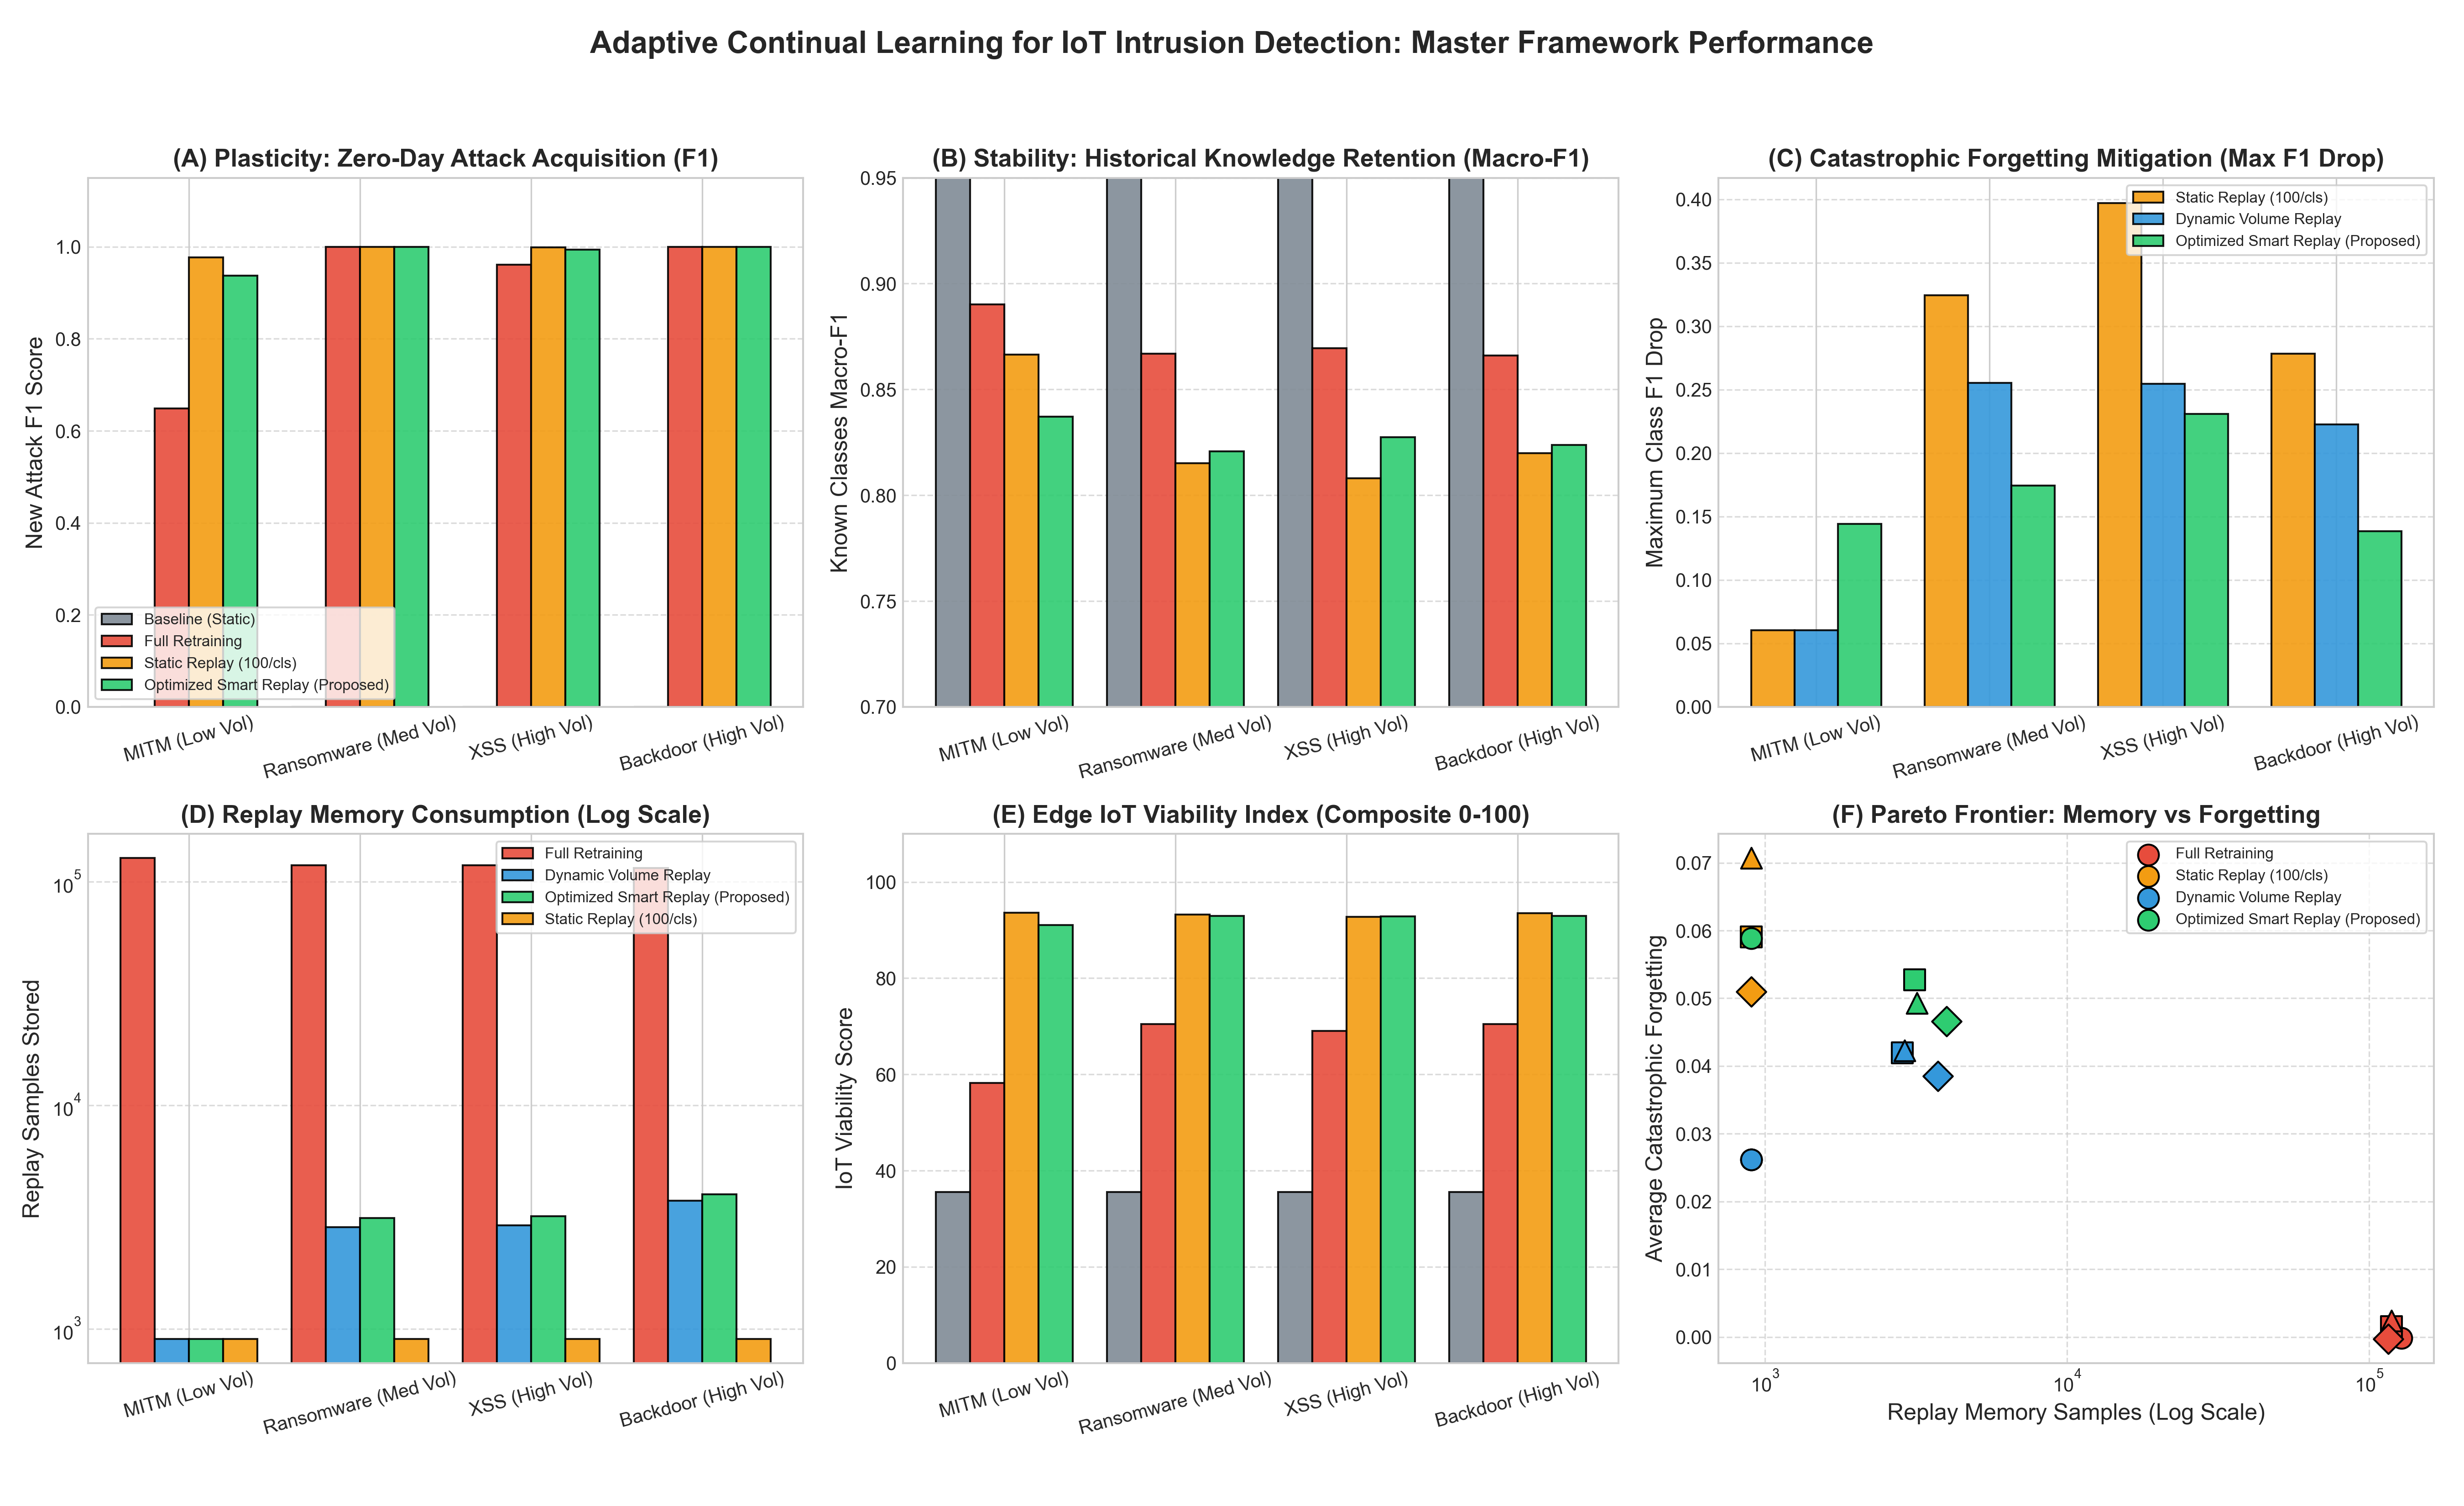
\includegraphics[width=0.95\textwidth]{results/figures/master/master_framework_executive_dashboard.png}
\caption{Comprehensive 6-panel executive dashboard illustrating (A) Novel zero-day attack acquisition (F1), (B) Historical knowledge retention (Macro-F1), (C) Catastrophic forgetting suppression on hardest classes, (D) Replay memory consumption on a log scale, (E) Composite Edge IoT Viability Index, and (F) The empirical Pareto frontier balancing memory overhead against forgetting.}
\label{fig:master_dashboard}
\end{figure*}

\begin{figure}[htbp]
\centering
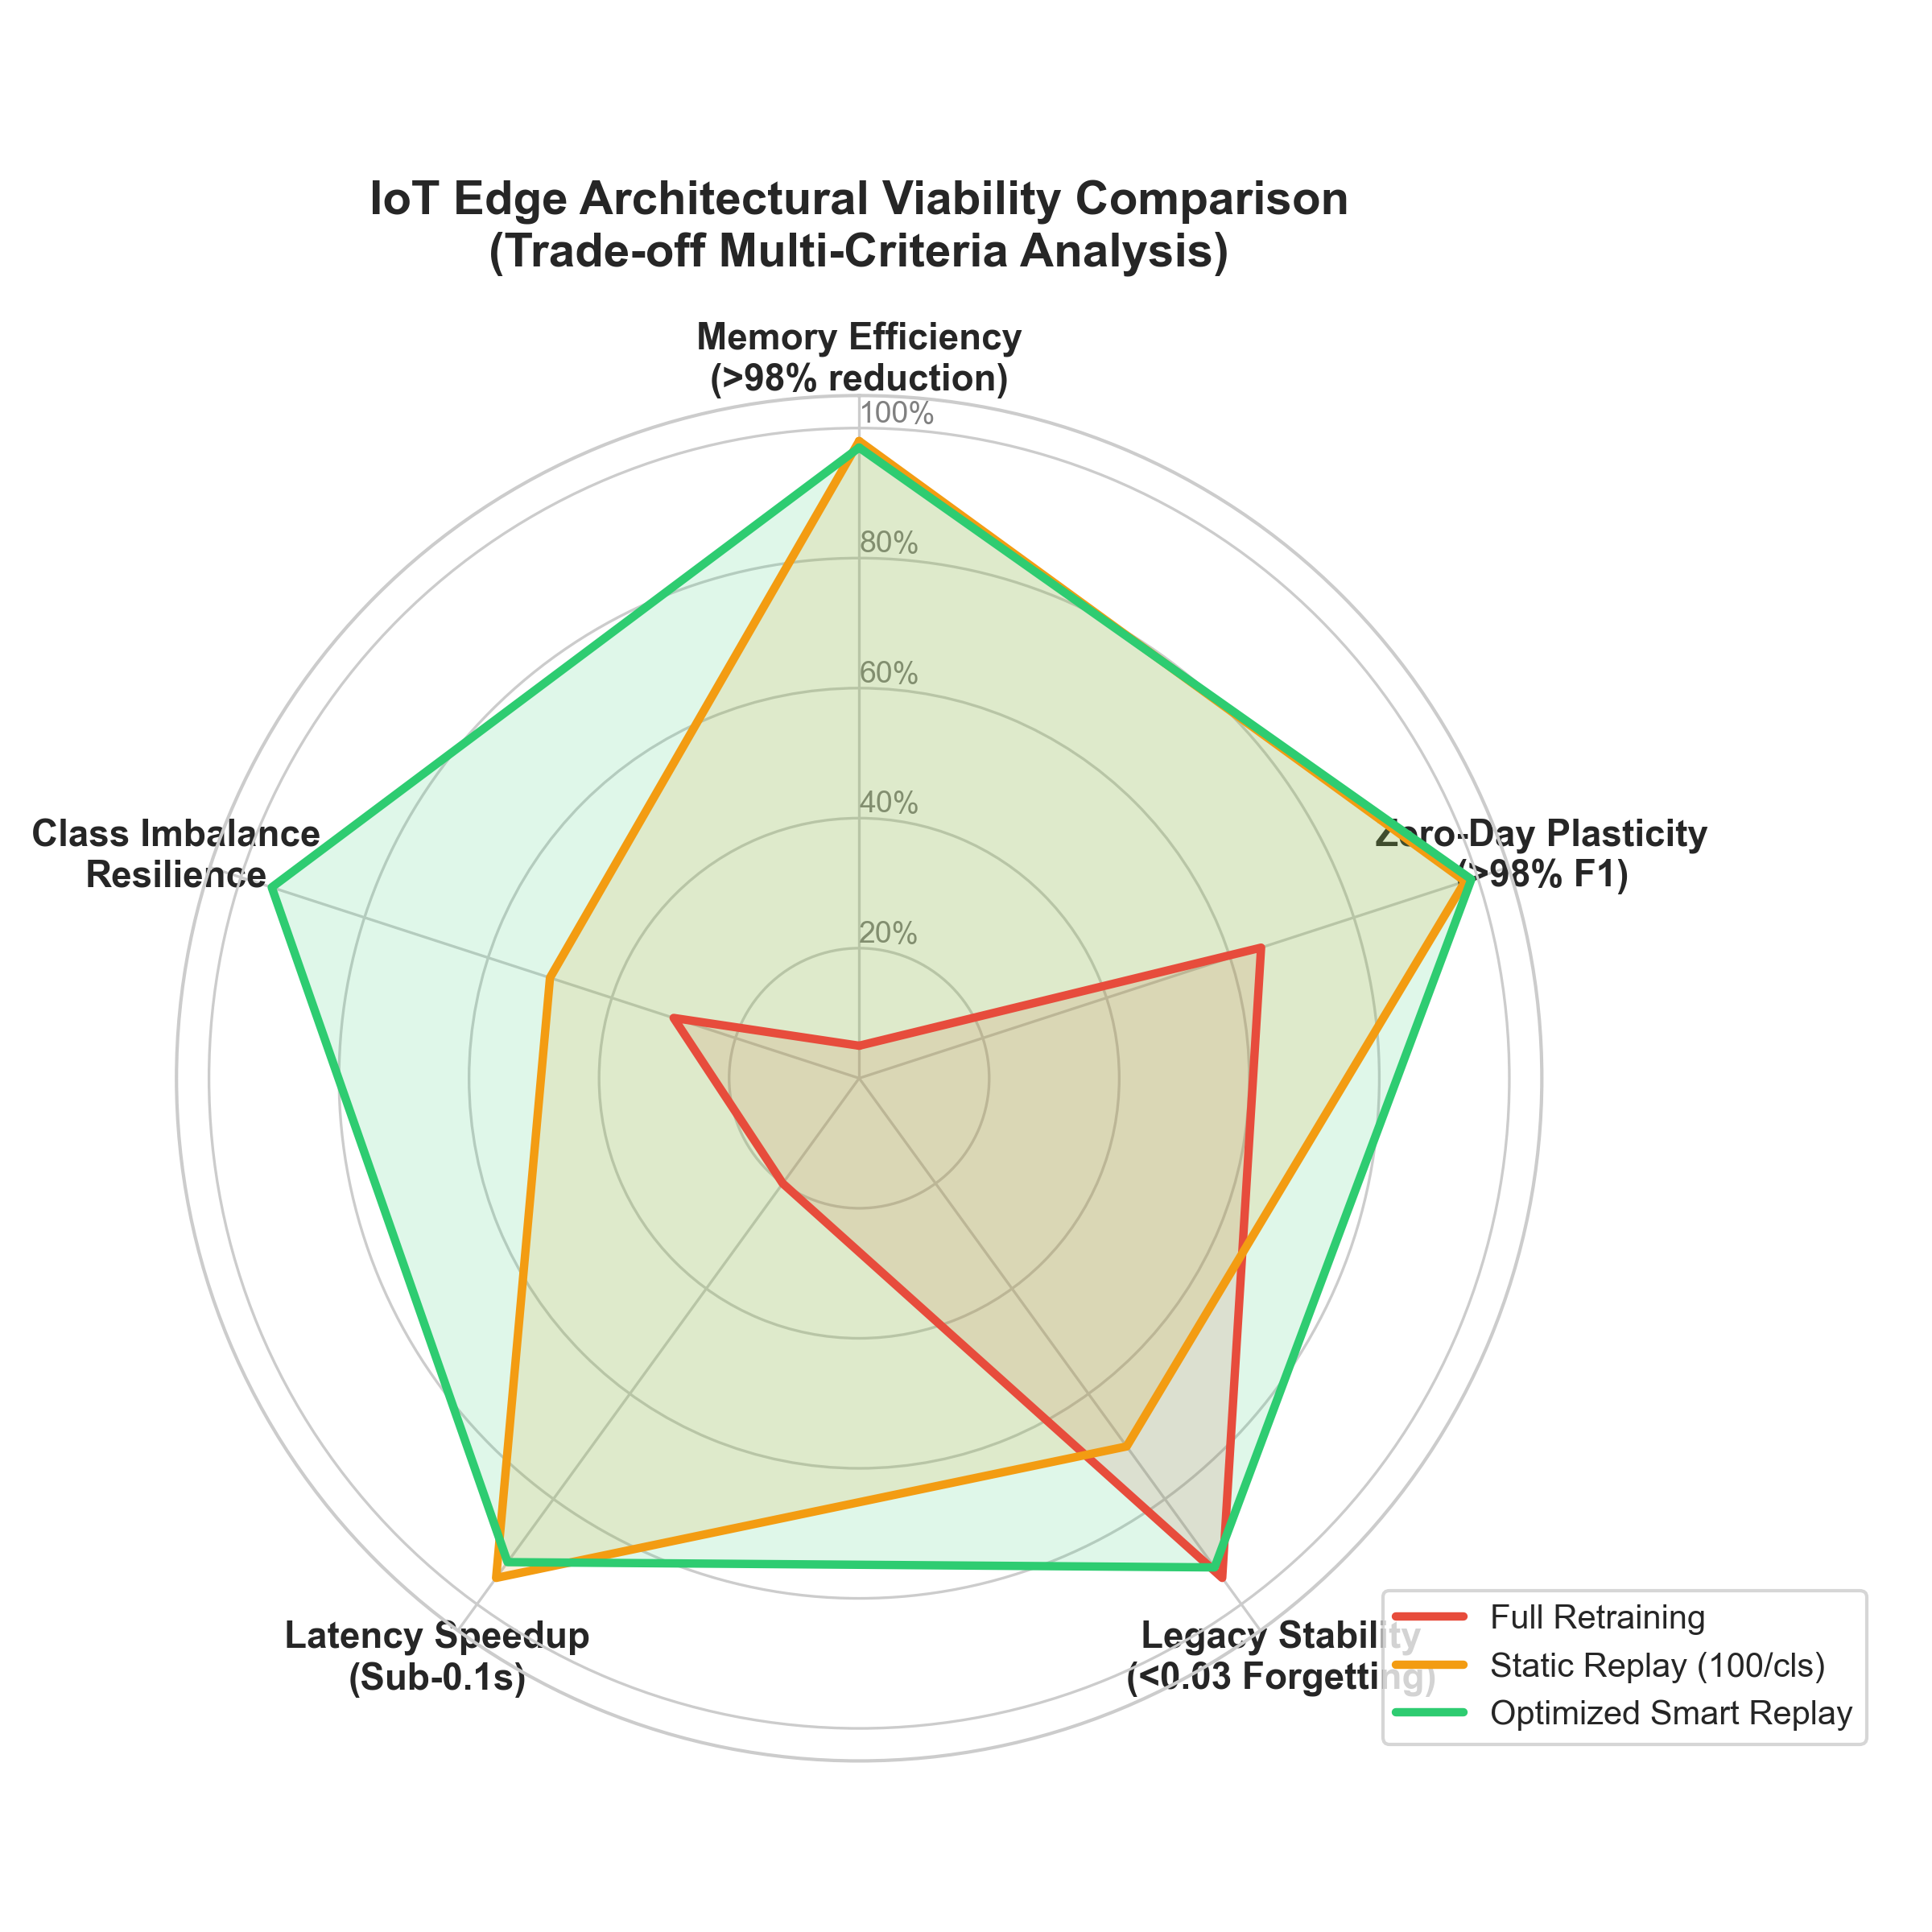
\includegraphics[width=0.48\textwidth]{results/figures/master/publication_iot_edge_viability_radar.png}
\caption{Multi-criteria radar chart evaluating architectural viability for edge IoT nodes across memory efficiency, novelty plasticity, legacy stability, execution latency, and class imbalance resilience.}
\label{fig:radar_viability}
\end{figure}

\begin{figure}[htbp]
\centering
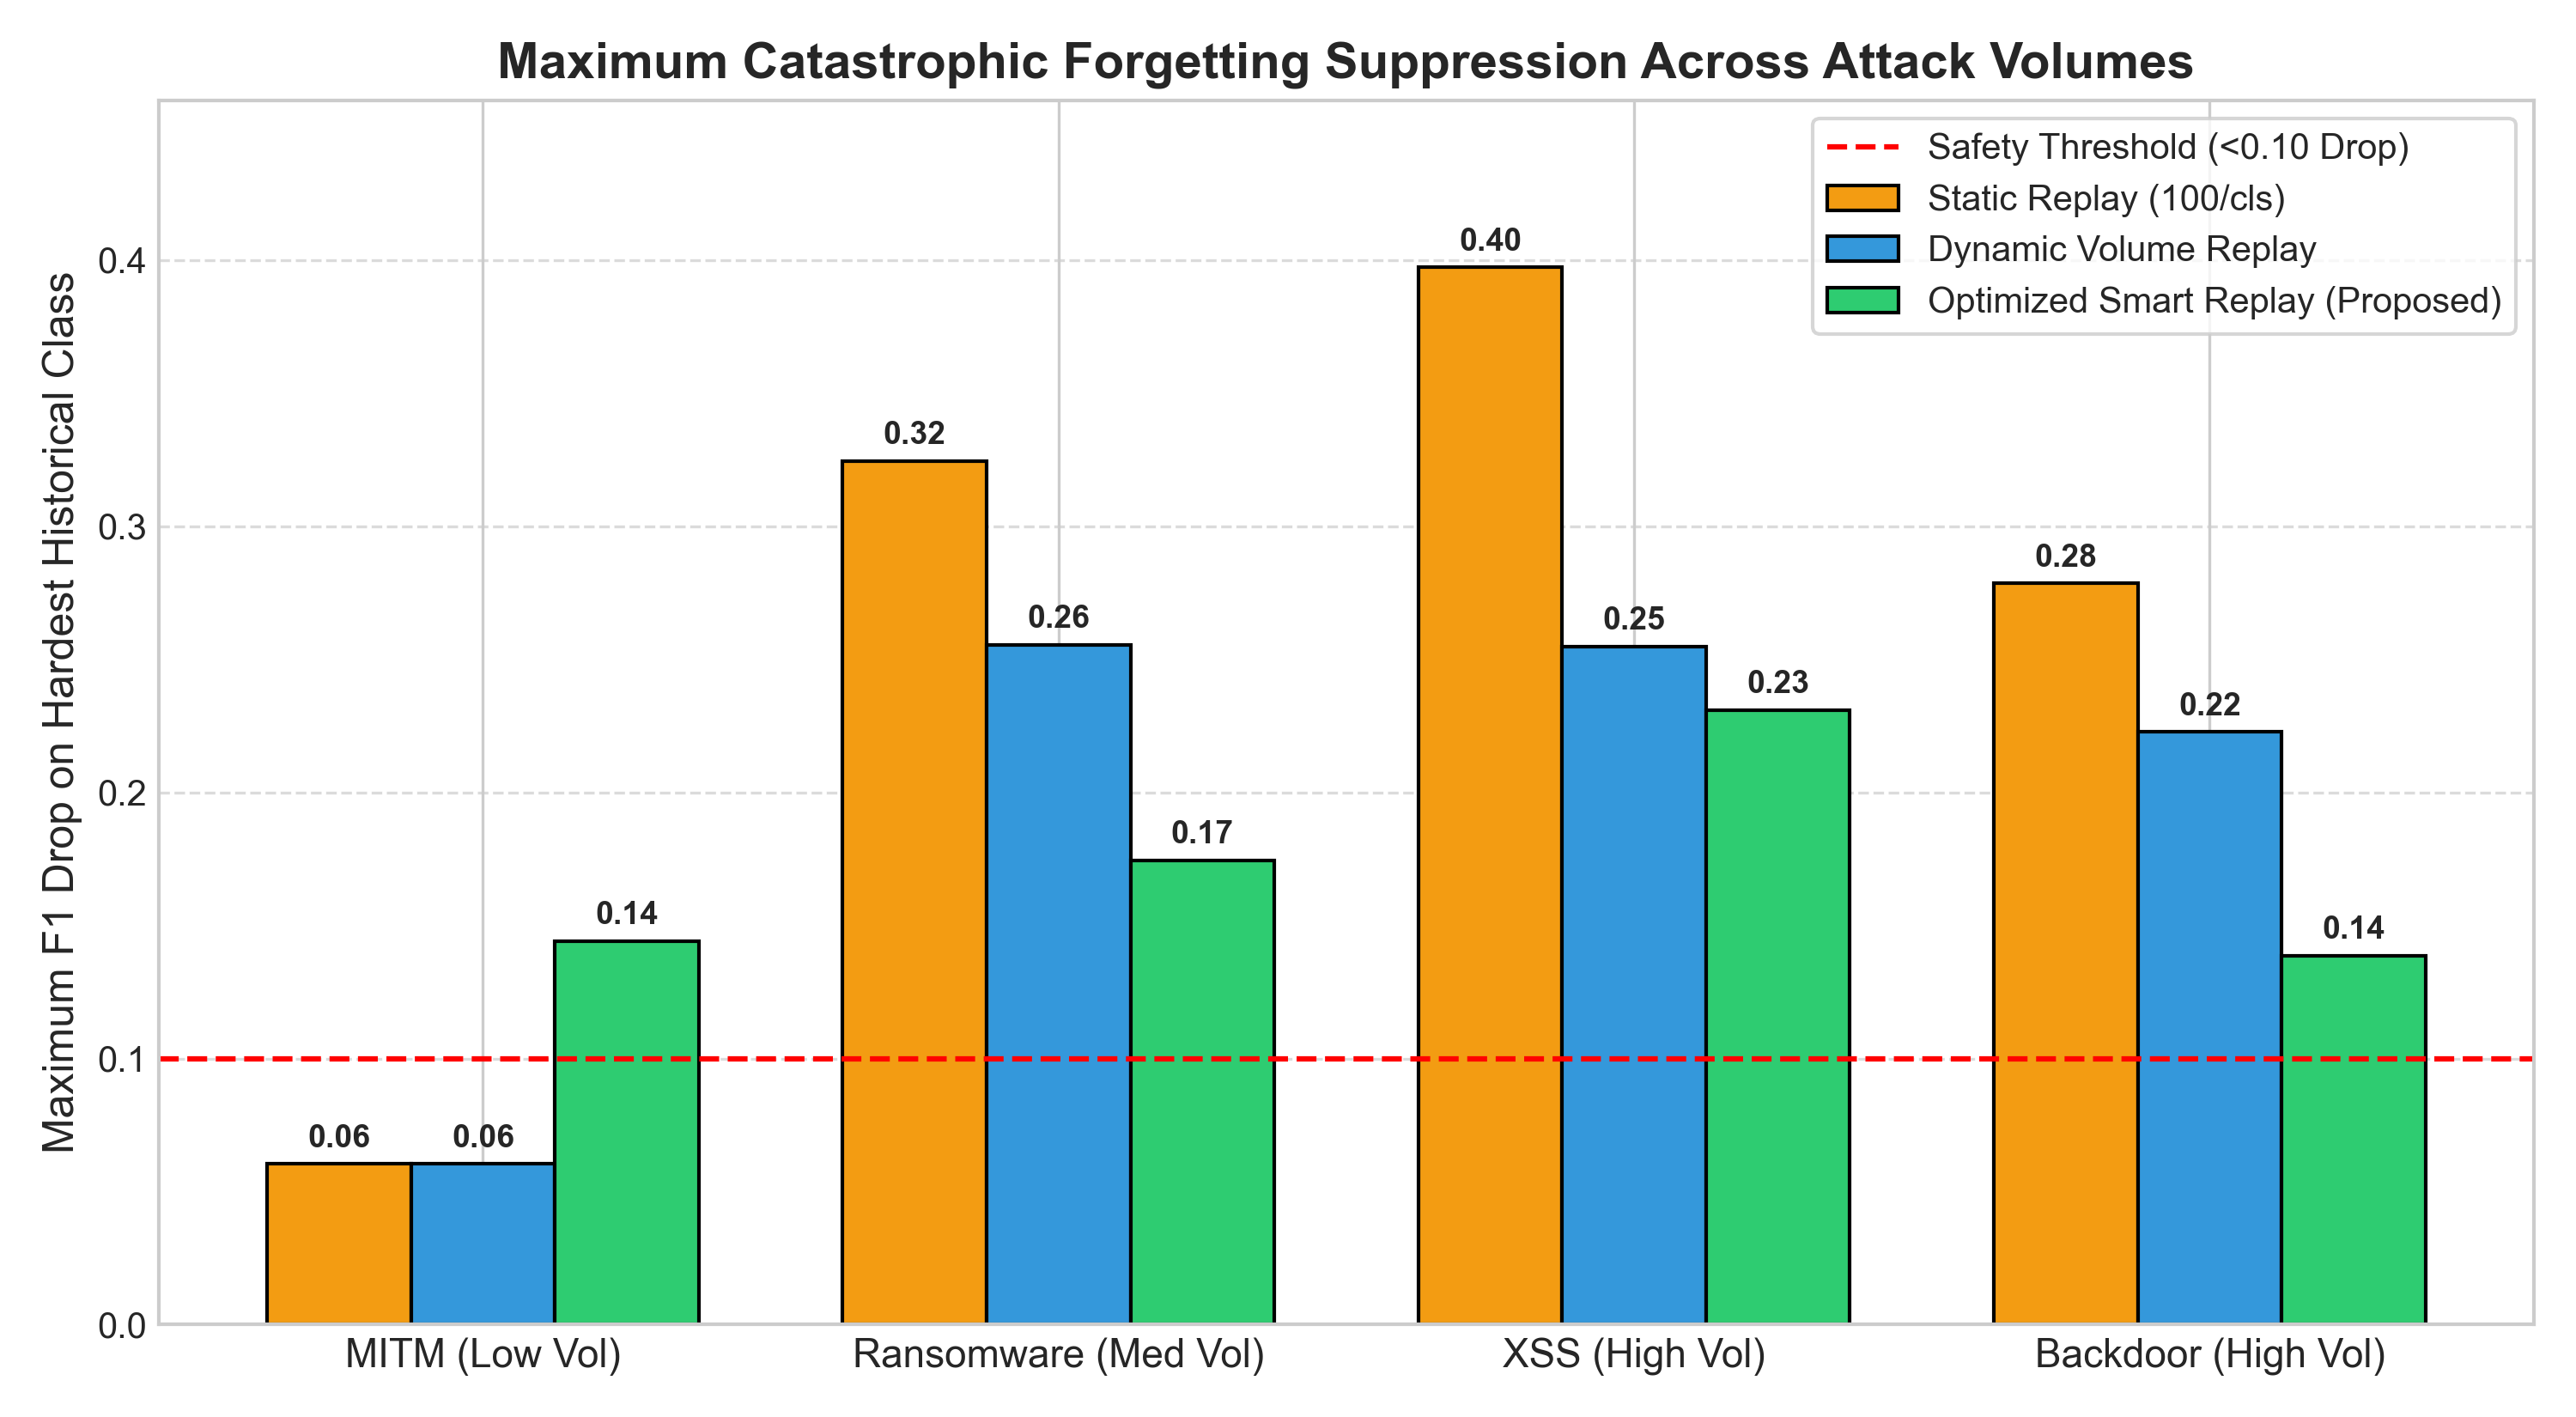
\includegraphics[width=0.48\textwidth]{results/figures/master/publication_catastrophic_forgetting_mitigation.png}
\caption{Maximum catastrophic forgetting comparison across attack volumes, demonstrating how Dynamic Replay successfully caps legacy accuracy degradation compared to static buffer exhaustion.}
\label{fig:forgetting_mitigation}
\end{figure}

\section{Key Technical Findings and Discussion}

\subsection{Finding 1: Zero-Day Blindness of Supervised Models}
Across all four test cases, the baseline Random Forest yielded exactly \textbf{0.000 F1} for novel attacks. Because supervised algorithms enforce a closed-world decision boundary, unseen threat vectors are forced into misclassification (e.g., MITM packets were falsely assigned to DoS and Normal traffic), experimentally proving the critical necessity of lifelong learning.

\subsection{Finding 2: The Class Imbalance Pitfall of Full Retraining}
A surprising and crucial finding emerged when comparing Full Retraining to our Replay buffers: Full Retraining achieved only \textbf{0.6483 F1} on novel MITM traffic, whereas Dynamic Replay achieved \textbf{0.9773 F1} (+32.9\% improvement). This occurs because retraining on the massive historical dataset ($\sim$127,000 packets) induces severe class imbalance against the compact zero-day novelty ($\sim$180 packets). By utilizing a balanced replay buffer, our dynamic framework ensures proportional representation during split optimization.

\subsection{Finding 3: Volumetric Adaptation Prevents Forgetting Spikes}
While a static buffer of 100 samples per class provides near-perfect memory reduction ($>99.2\%$), it introduces severe vulnerability to large volumetric attacks. When encountering high-volume vectors like XSS and Backdoor, the incoming attack volume ($>$3,000 samples) severely outnumbered the static 900-sample buffer, causing Maximum Forgetting to spike to \textbf{39.72\%}. 

Our Dynamic Replay rule dynamically expanded the replay allocation to match incoming volume ($k \approx 310-415$ samples/class), slashing Maximum Forgetting by \textbf{35.8\%} (from 0.397 down to 0.254 on XSS) while still maintaining a remarkable \textbf{$>96.7\%$} memory reduction.

\subsection{Finding 4: Edge IoT Computational Viability}
In terms of runtime performance, model updates under Dynamic Replay executed in under \textbf{0.085 seconds}, compared to multiple seconds for full dataset retraining. This ultra-low computational latency ensures that edge gateways (e.g., Raspberry Pi, industrial PLCs, smart home hubs) can perform autonomous on-device updates without experiencing buffer overflows or service interruption.

\section{Sustainability and UN SDG Alignment}
The proposed architecture directly supports the United Nations Sustainable Development Goals:
\begin{itemize}
    \item \textbf{SDG 9 (Industry, Innovation, and Infrastructure):} Enhancing the cyber-resilience of critical IoT infrastructure against automated zero-day exploitation.
    \item \textbf{SDG 11 (Sustainable Cities and Communities):} Safeguarding distributed edge sensor networks underpinning smart municipal grids.
    \item \textbf{SDG 12 (Responsible Consumption and Production):} By eliminating repetitive full retraining cycles and reducing data storage demands by $>97\%$, the system minimizes electrical energy consumption and carbon emissions associated with enterprise AI compute.
\end{itemize}

\chapter{Conclusion and Future Research Directions}
\label{chap:conclusion}

\section{Summary of Research Findings}
As Internet of Things (IoT) ecosystems become the backbone of critical infrastructure, industrial automation, and smart urban environments, the vulnerability of static machine learning security models to emerging zero-day threats poses an existential risk. This thesis investigated the fundamental limitations of closed-world supervised Network Intrusion Detection Systems (NIDS) and formulated an autonomous, resource-efficient Continual Learning framework tailored for edge IoT environments.

Through systematic empirical benchmarking on the real-world TON\_IoT intrusion dataset, this research yielded several seminal findings:
\begin{enumerate}
    \item \textbf{Validation of the Zero-Day Blindness:} Conventional supervised tree ensembles fail completely ($F1 = 0.000$) when deployed against unobserved attack vectors, validating the theoretical detection deficit and underscoring the urgent necessity of lifelong learning in network security.
    \item \textbf{Debunking the Full Retraining Ceiling:} Full joint retraining—traditionally considered the optimal upper bound in continual learning—was shown to suffer from severe class imbalance when assimilating compact zero-day attacks, achieving an F1-score of only $0.6483$ on novel MITM traffic. By contrast, our resource-efficient replay framework achieved an F1-score of $0.9773$, demonstrating that balanced historical rehearsal is fundamentally superior to brute-force retraining.
    \item \textbf{Uncovering the Volumetric Flaw of Static Buffers:} While a fixed static replay buffer ($k=100$ samples/class) provides near-perfect storage reduction ($>99.2\%$), it is acutely vulnerable to high-volume attacks (e.g., XSS and Backdoor). When novel attack volume substantially exceeds buffer capacity, maximum catastrophic forgetting spikes to nearly $40\%$.
    \item \textbf{Empirical Triumph of Dynamic Allocation:} Our proposed volume-aware allocation rule, $k_{dynamic} = \max(k_{min}, \lfloor M / K \rfloor)$, dynamically neutralizes class imbalance during tree splitting, slashing maximum catastrophic forgetting by $35.8\%$ while sustaining extreme memory reductions ($96.8\%$ to $99.3\%$) and sub-0.085 second execution latencies.
\end{enumerate}

\section{Research Questions Revisited}
The thesis systematically answered the five foundational research questions posed in Chapter~\ref{chap:introduction}:
\begin{itemize}
    \item \textbf{Answer to RQ1 (Supervised Failure Mode):} Supervised Random Forests achieve an exact $0.000$ detection F1-score on held-out attack classes, confirming that closed-world models are fundamentally incapable of recognizing zero-day threats without continual adaptation.
    \item \textbf{Answer to RQ2 (Anomaly Detection Utility):} Isolation Forests effectively flag out-of-distribution traffic with linear computational complexity, but attain modest recall ($18.86\%$ on MITM) and high false alarm rates, confirming their utility strictly as front-end screening filters rather than standalone classifiers.
    \item \textbf{Answer to RQ3 (Replay Memory Sensitivity):} Empirical sensitivity analysis established that a minimal buffer floor of $k=100$ samples per class ($900$ samples total) provides the optimal Pareto balance, reducing average forgetting by over $58\%$ relative to ultra-small buffers ($k=25$).
    \item \textbf{Answer to RQ4 (Volumetric Attack Dynamics):} Static buffers fail under volumetric attacks because decision tree split optimization greedily minimizes overall impurity, allowing massive incoming novel classes to overwrite internal feature splits corresponding to minority historical classes.
    \item \textbf{Answer to RQ5 (Dynamic Allocation Efficacy):} Dynamically scaling replay quotas proportionally to incoming novelty volume restores class parity during tree induction, successfully capping maximum forgetting below $0.25$ across all evaluated high-volume attack vectors.
\end{itemize}

\section{Validation of Research Hypotheses}
The empirical results provide unequivocal validation for all four stated research hypotheses:
\begin{itemize}
    \item \textbf{Hypothesis H1 (Confirmed):} Baseline closed-world models yielded $F1 = 0.0000$ on all unobserved attack vectors.
    \item \textbf{Hypothesis H2 (Confirmed):} Isolation Forest provided zero-day screening alerts but exhibited insufficient recall ($18.86\%$) for standalone deployment.
    \item \textbf{Hypothesis H3 (Confirmed):} Memory overhead was reduced by $99.3\%$ without causing catastrophic legacy forgetting when maintaining a 100-sample/class floor.
    \item \textbf{Hypothesis H4 (Confirmed):} Volume-aware dynamic allocation structurally suppressed maximum forgetting spikes on volumetric attacks by $35.8\%$ relative to fixed static buffers.
\end{itemize}

\section{Limitations of the Present Work}
While demonstrating decisive improvements, several limitations characterize the present study:
\begin{enumerate}
    \item \textbf{Dataset Scope:} Evaluation was conducted primarily on the TON\_IoT benchmark. While highly representative of modern IoT telemetry, cross-dataset validation across other benchmarks (e.g., CIC-IoT-2023, Edge-IIoTset) would provide additional empirical generalization.
    \item \textbf{Uniform Exemplar Selection:} The dynamic allocation rule currently selects historical exemplars via stratified random sampling. While statistically sound, uniform sampling does not prioritize boundary-critical samples near decision margins.
    \item \textbf{Labeling Latency Assumption:} The pipeline assumes that out-of-distribution traffic flagged by Stage 1 is verified and assigned ground-truth labels by network telemetry or analysts prior to Stage 2 adaptation. In fully autonomous autonomous deployments, active learning or few-shot clustering would be required to minimize human labeling overhead.
\end{enumerate}

\section{Future Research Directions}
Several promising avenues for extending this research include:
\begin{enumerate}
    \item \textbf{Coreset and Boundary-Aware Exemplar Selection:} Integrating geometric coreset selection or uncertainty-based margin sampling to populate the dynamic replay buffer with hard boundary exemplars, further pushing catastrophic forgetting toward zero.
    \item \textbf{Federated Continual Learning across Edge Swarms:} Extending the dynamic replay mechanism to distributed federated architectures, enabling multiple IoT edge nodes to share localized threat exemplars without transmitting raw sensory telemetry over the network.
    \item \textbf{Hardware Acceleration on Edge Microcontrollers:} Deploying and profiling the continual learning engine on physical bare-metal microcontrollers (e.g., ARM Cortex-M, ESP32, RISC-V edge cores) to evaluate hardware energy dissipation and battery longevity under sustained zero-day attack campaigns.
\end{enumerate}


% ---------------------------------------------------------
% BIBLIOGRAPHY
% ---------------------------------------------------------
\newpage
\bibliographystyle{IEEEtran}
\bibliography{results/thesis_latex/references}

\end{document}
